
% This LaTeX was auto-generated from an M-file by MATLAB.
% To make changes, update the M-file and republish this document.

\documentclass{article}
\usepackage{graphicx}
\usepackage{color}

\sloppy
\definecolor{lightgray}{gray}{0.5}
\setlength{\parindent}{0pt}

\title{Diffusion Maps Tutorial}
\date{}

\begin{document}

\maketitle
    
\subsection*{Contents}

\begin{itemize}
\setlength{\itemsep}{-1ex}
   \item Create Data Set
   \item Compute Distance Matrix
   \item Calculate Kernel Matrix
   \item Compute Diffusion Matrix
   \item Calculate Eigenvectors and Eigenvalues
   \item Order Data by First (nontrivial) Diffusion Maps Eigenvector
\end{itemize}
\begin{verbatim}
clear all
close all
\end{verbatim}


\subsection*{Create Data Set}

\begin{par}
First, we create an artifical data set \texttt{x} of $n=7$ data points which lie on a one-dimensional curve in two dimensions. This data set can be parameterized by t he angular direction $\theta$.
\end{par} \vspace{1em}
\begin{verbatim}
n = 7;

theta = linspace(0, 3*pi/2, n);

x = [0.9*cos(theta); 0.9*sin(theta)]

figure;
scatter(x(1,:),x(2,:),200, 'k', '.');
xlabel('x(1)');
ylabel('x(2)');
\end{verbatim}

        \color{lightgray} \begin{verbatim}
x =

    0.9000    0.6364    0.0000   -0.6364   -0.9000   -0.6364   -0.0000
         0    0.6364    0.9000    0.6364    0.0000   -0.6364   -0.9000

\end{verbatim} \color{black}
    
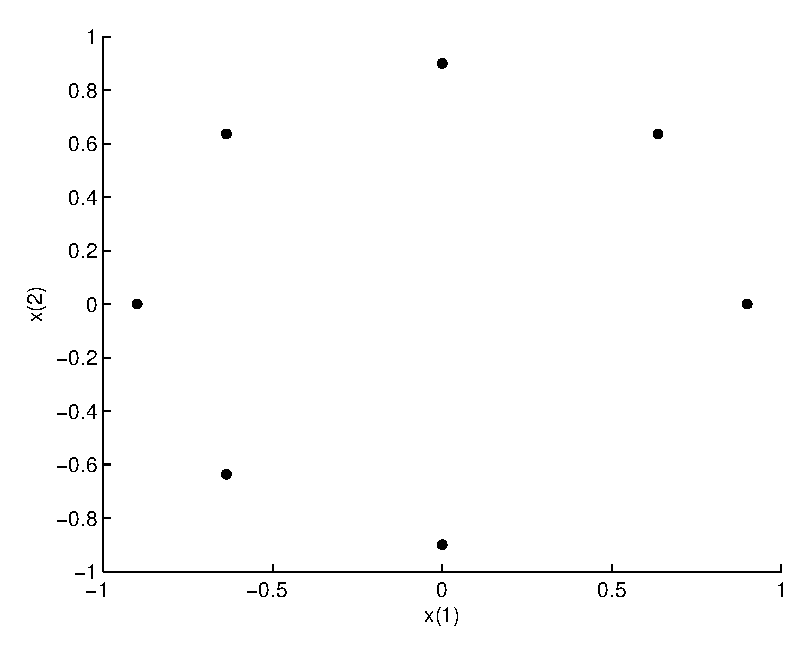
\includegraphics [width=4in]{diffusion_maps_tutorial_01.eps}


\subsection*{Compute Distance Matrix}

\begin{par}
Then we compute the $n \times n$ distance matrix \texttt{dist\_matrix} between data points where \texttt{dist\_matrix(i,j)} is the distance between data point $i$ and data point $j$. Assuming the data points are stored in columns, this can be done using the \texttt{dist} function.
\end{par} \vspace{1em}
\begin{verbatim}
dist_matrix = dist(x)
\end{verbatim}

        \color{lightgray} \begin{verbatim}
dist_matrix =

         0    0.6888    1.2728    1.6630    1.8000    1.6630    1.2728
    0.6888         0    0.6888    1.2728    1.6630    1.8000    1.6630
    1.2728    0.6888         0    0.6888    1.2728    1.6630    1.8000
    1.6630    1.2728    0.6888         0    0.6888    1.2728    1.6630
    1.8000    1.6630    1.2728    0.6888         0    0.6888    1.2728
    1.6630    1.8000    1.6630    1.2728    0.6888         0    0.6888
    1.2728    1.6630    1.8000    1.6630    1.2728    0.6888         0

\end{verbatim} \color{black}
    

\subsection*{Calculate Kernel Matrix}

\begin{par}
We then compute the $n \times n$ matrix $W$, with $$ W_{ij} = \exp \left(-\frac{ \| x_i - x_j \|^2}{\epsilon^2} \right) $$ where $\epsilon$, the kernel scale, is a characteristic distance within the data set. We typically set $\epsilon$ to be some fraction of the median of the pairwise distances. Here we take $\epsilon$ as half the median of the pairwise distances.
\end{par} \vspace{1em}
\begin{verbatim}
eps = median(dist_matrix(:))/2

W = exp(-dist_matrix.^2/eps.^2)
\end{verbatim}

        \color{lightgray} \begin{verbatim}
eps =

    0.6364


W =

    1.0000    0.3099    0.0183    0.0011    0.0003    0.0011    0.0183
    0.3099    1.0000    0.3099    0.0183    0.0011    0.0003    0.0011
    0.0183    0.3099    1.0000    0.3099    0.0183    0.0011    0.0003
    0.0011    0.0183    0.3099    1.0000    0.3099    0.0183    0.0011
    0.0003    0.0011    0.0183    0.3099    1.0000    0.3099    0.0183
    0.0011    0.0003    0.0011    0.0183    0.3099    1.0000    0.3099
    0.0183    0.0011    0.0003    0.0011    0.0183    0.3099    1.0000

\end{verbatim} \color{black}
    

\subsection*{Compute Diffusion Matrix}

\begin{par}
We then compute the $n \times n$ diaganol matrix $D$, with $$ D_{ii} = \sum_{j=1}^n W_{ij} $$ and the $n \times n$ matrix $$A = D^{-1}W. $$
\end{par} \vspace{1em}
\begin{verbatim}
D = diag(sum(W))

A = inv(D)*W
\end{verbatim}

        \color{lightgray} \begin{verbatim}
D =

    1.3490         0         0         0         0         0         0
         0    1.6406         0         0         0         0         0
         0         0    1.6578         0         0         0         0
         0         0         0    1.6586         0         0         0
         0         0         0         0    1.6578         0         0
         0         0         0         0         0    1.6406         0
         0         0         0         0         0         0    1.3490


A =

    0.7413    0.2297    0.0136    0.0008    0.0002    0.0008    0.0136
    0.1889    0.6095    0.1889    0.0112    0.0007    0.0002    0.0007
    0.0110    0.1869    0.6032    0.1869    0.0110    0.0007    0.0002
    0.0007    0.0110    0.1868    0.6029    0.1868    0.0110    0.0007
    0.0002    0.0007    0.0110    0.1869    0.6032    0.1869    0.0110
    0.0007    0.0002    0.0007    0.0112    0.1889    0.6095    0.1889
    0.0136    0.0008    0.0002    0.0008    0.0136    0.2297    0.7413

\end{verbatim} \color{black}
    

\subsection*{Calculate Eigenvectors and Eigenvalues}

\begin{par}
We then compute the top eigenvectors and eigenvalues of $A$, and order them by the magnitude of the eigenvalues.
\end{par} \vspace{1em}
\begin{verbatim}
% compute eigenvectors and eigenvalues
[evecs, evals] = eig(A);

% sort eigenvectors and eigenvalues
[~, I] = sort(abs(diag(evals)), 'descend');
evecs = evecs(:,I)
evals = evals(I,I)
\end{verbatim}

        \color{lightgray} \begin{verbatim}
evecs =

   -0.3780   -0.4976    0.5021   -0.4755    0.3897   -0.2997   -0.1512
   -0.3780   -0.4344    0.1539    0.1544   -0.4454    0.5098    0.3396
   -0.3780   -0.2523   -0.3041    0.5001   -0.1334   -0.3876   -0.4745
   -0.3780    0.0000   -0.5134    0.0000    0.5137   -0.0000    0.5227
   -0.3780    0.2523   -0.3041   -0.5001   -0.1334    0.3876   -0.4745
   -0.3780    0.4344    0.1539   -0.1544   -0.4454   -0.5098    0.3396
   -0.3780    0.4976    0.5021    0.4755    0.3897    0.2997   -0.1512


evals =

    1.0000         0         0         0         0         0         0
         0    0.9343         0         0         0         0         0
         0         0    0.8163         0         0         0         0
         0         0         0    0.6394         0         0         0
         0         0         0         0    0.4878         0         0
         0         0         0         0         0    0.3556         0
         0         0         0         0         0         0    0.2777

\end{verbatim} \color{black}
    

\subsection*{Order Data by First (nontrivial) Diffusion Maps Eigenvector}

\begin{par}
The first eigenvector is a trivial constant eigenvector with eigenvalue 1. The second eigenvector provides an ordering of the data. As expected, we see The second eigenvector is one-to-one with the $\theta$, which parameterizes the arclength along the curve. Furthermore, if we color the data by the value of this second eigenvector, we can see that this eigenvector does order the data along the one-dimensional nonlinear curve.
\end{par} \vspace{1em}
\begin{verbatim}
figure;
scatter(theta, evecs(:,2), 50, 'k')
xlabel('\theta (parameterizes arclength along curve)')
ylabel('first diffusion maps coordinate')

figure;
scatter(x(1,:),x(2,:),200, evecs(:,2), '.');
xlabel('x(1)');
ylabel('x(2)');
h = colorbar;
ylabel(h, 'first diffusion maps coordinate')
\end{verbatim}

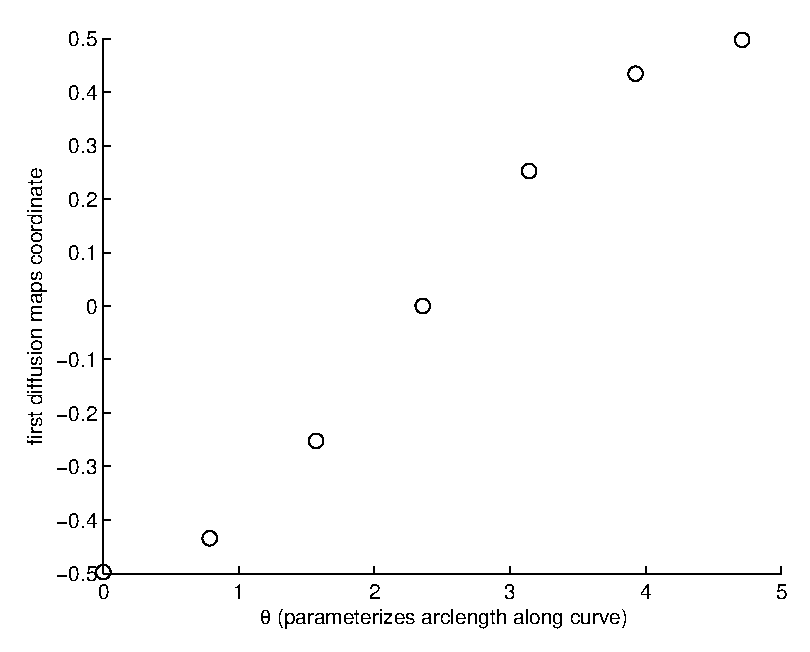
\includegraphics [width=4in]{diffusion_maps_tutorial_02.eps}

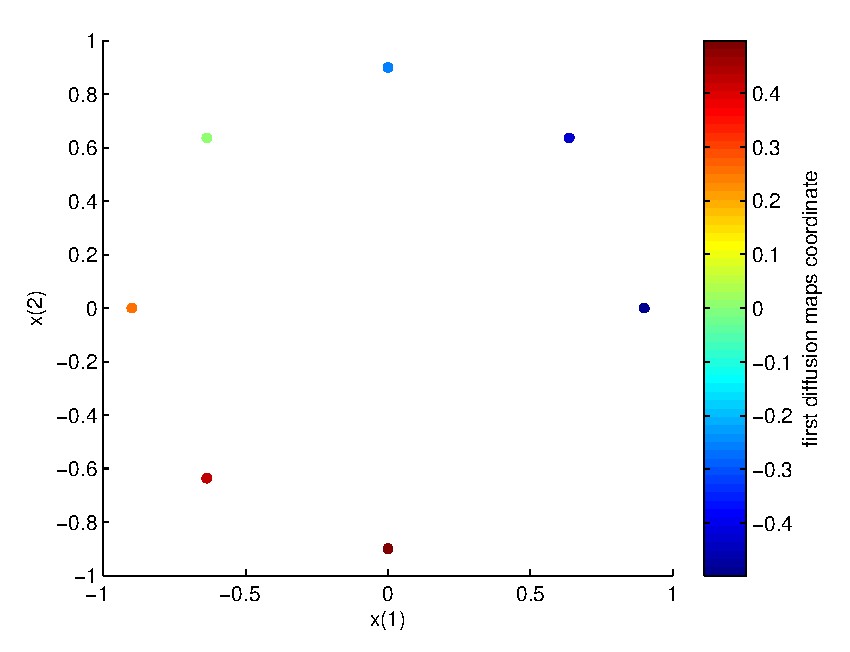
\includegraphics [width=4in]{diffusion_maps_tutorial_03.eps}



\end{document}
    
